\section{系统需求分析、设计与实现}\label{sec:system}

\subsection{系统建设目标}

系统部分的目标很明确：不做生产级大平台，而是实现一套能在本地真实运行、能用于答辩演示，并且可以承接前文实验结果的轻量级检测系统。它需要覆盖前端、后端、数据库和算法接入几个环节，但实现规模要控制在本科毕业设计可维护的范围内。

最终方案采用 React + FastAPI + SQLite 的本地单机架构。React 负责任务提交、状态查询和结果展示；FastAPI 便于组织 HTTP 接口，并能直接调用 Python 推理代码；SQLite 保存任务、结果和产物路径，不需要额外部署数据库服务。这个组合启动成本低、调试路径短，同时仍能体现较完整的前后端和持久化设计。

\subsection{系统需求分析}

\subsubsection{功能需求}

结合课题任务和答辩演示，系统需要覆盖以下功能。

\begin{enumerate}
  \item \textbf{模型管理}：读取模型配置，展示模型名称、状态和权重信息，并支持模型启用或停用；
  \item \textbf{任务提交}：支持单张图像与批量图像上传，并允许用户设置推理模式、模型类型和置信度阈值；
  \item \textbf{任务执行}：以异步方式执行推理任务，避免前端界面阻塞，并支持任务状态查询；
  \item \textbf{结果展示}：展示检测框可视化图像、结构化检测结果表格及统计信息；
  \item \textbf{结果持久化}：系统重启后仍保留历史任务、结果和输出文件路径，支持回放与复查。
\end{enumerate}

\subsubsection{非功能需求}

非功能需求来自实际调试和演示。环境安装、数据库初始化和项目启动方式需要可重复；算法层、服务层和展示层的边界要清楚，后续替换模型时不至于牵动整套页面；界面信息要适合答辩现场快速展示；同时避免 Redis、Celery 或分布式组件等超出本课题规模的依赖，降低部署和排错成本。

\subsection{系统总体架构}

系统采用前后端分离架构，如图~\ref{fig:ch5_architecture} 所示。前端处理任务创建、列表查询和结果可视化；后端提供接口服务、任务调度、状态管理和静态文件访问；数据库保存模型、任务、检测结果和输出文件路径；算法部分复用已有推理内核，并由后端通过统一接口调用。

\begin{figure}[htbp]
  \centering
  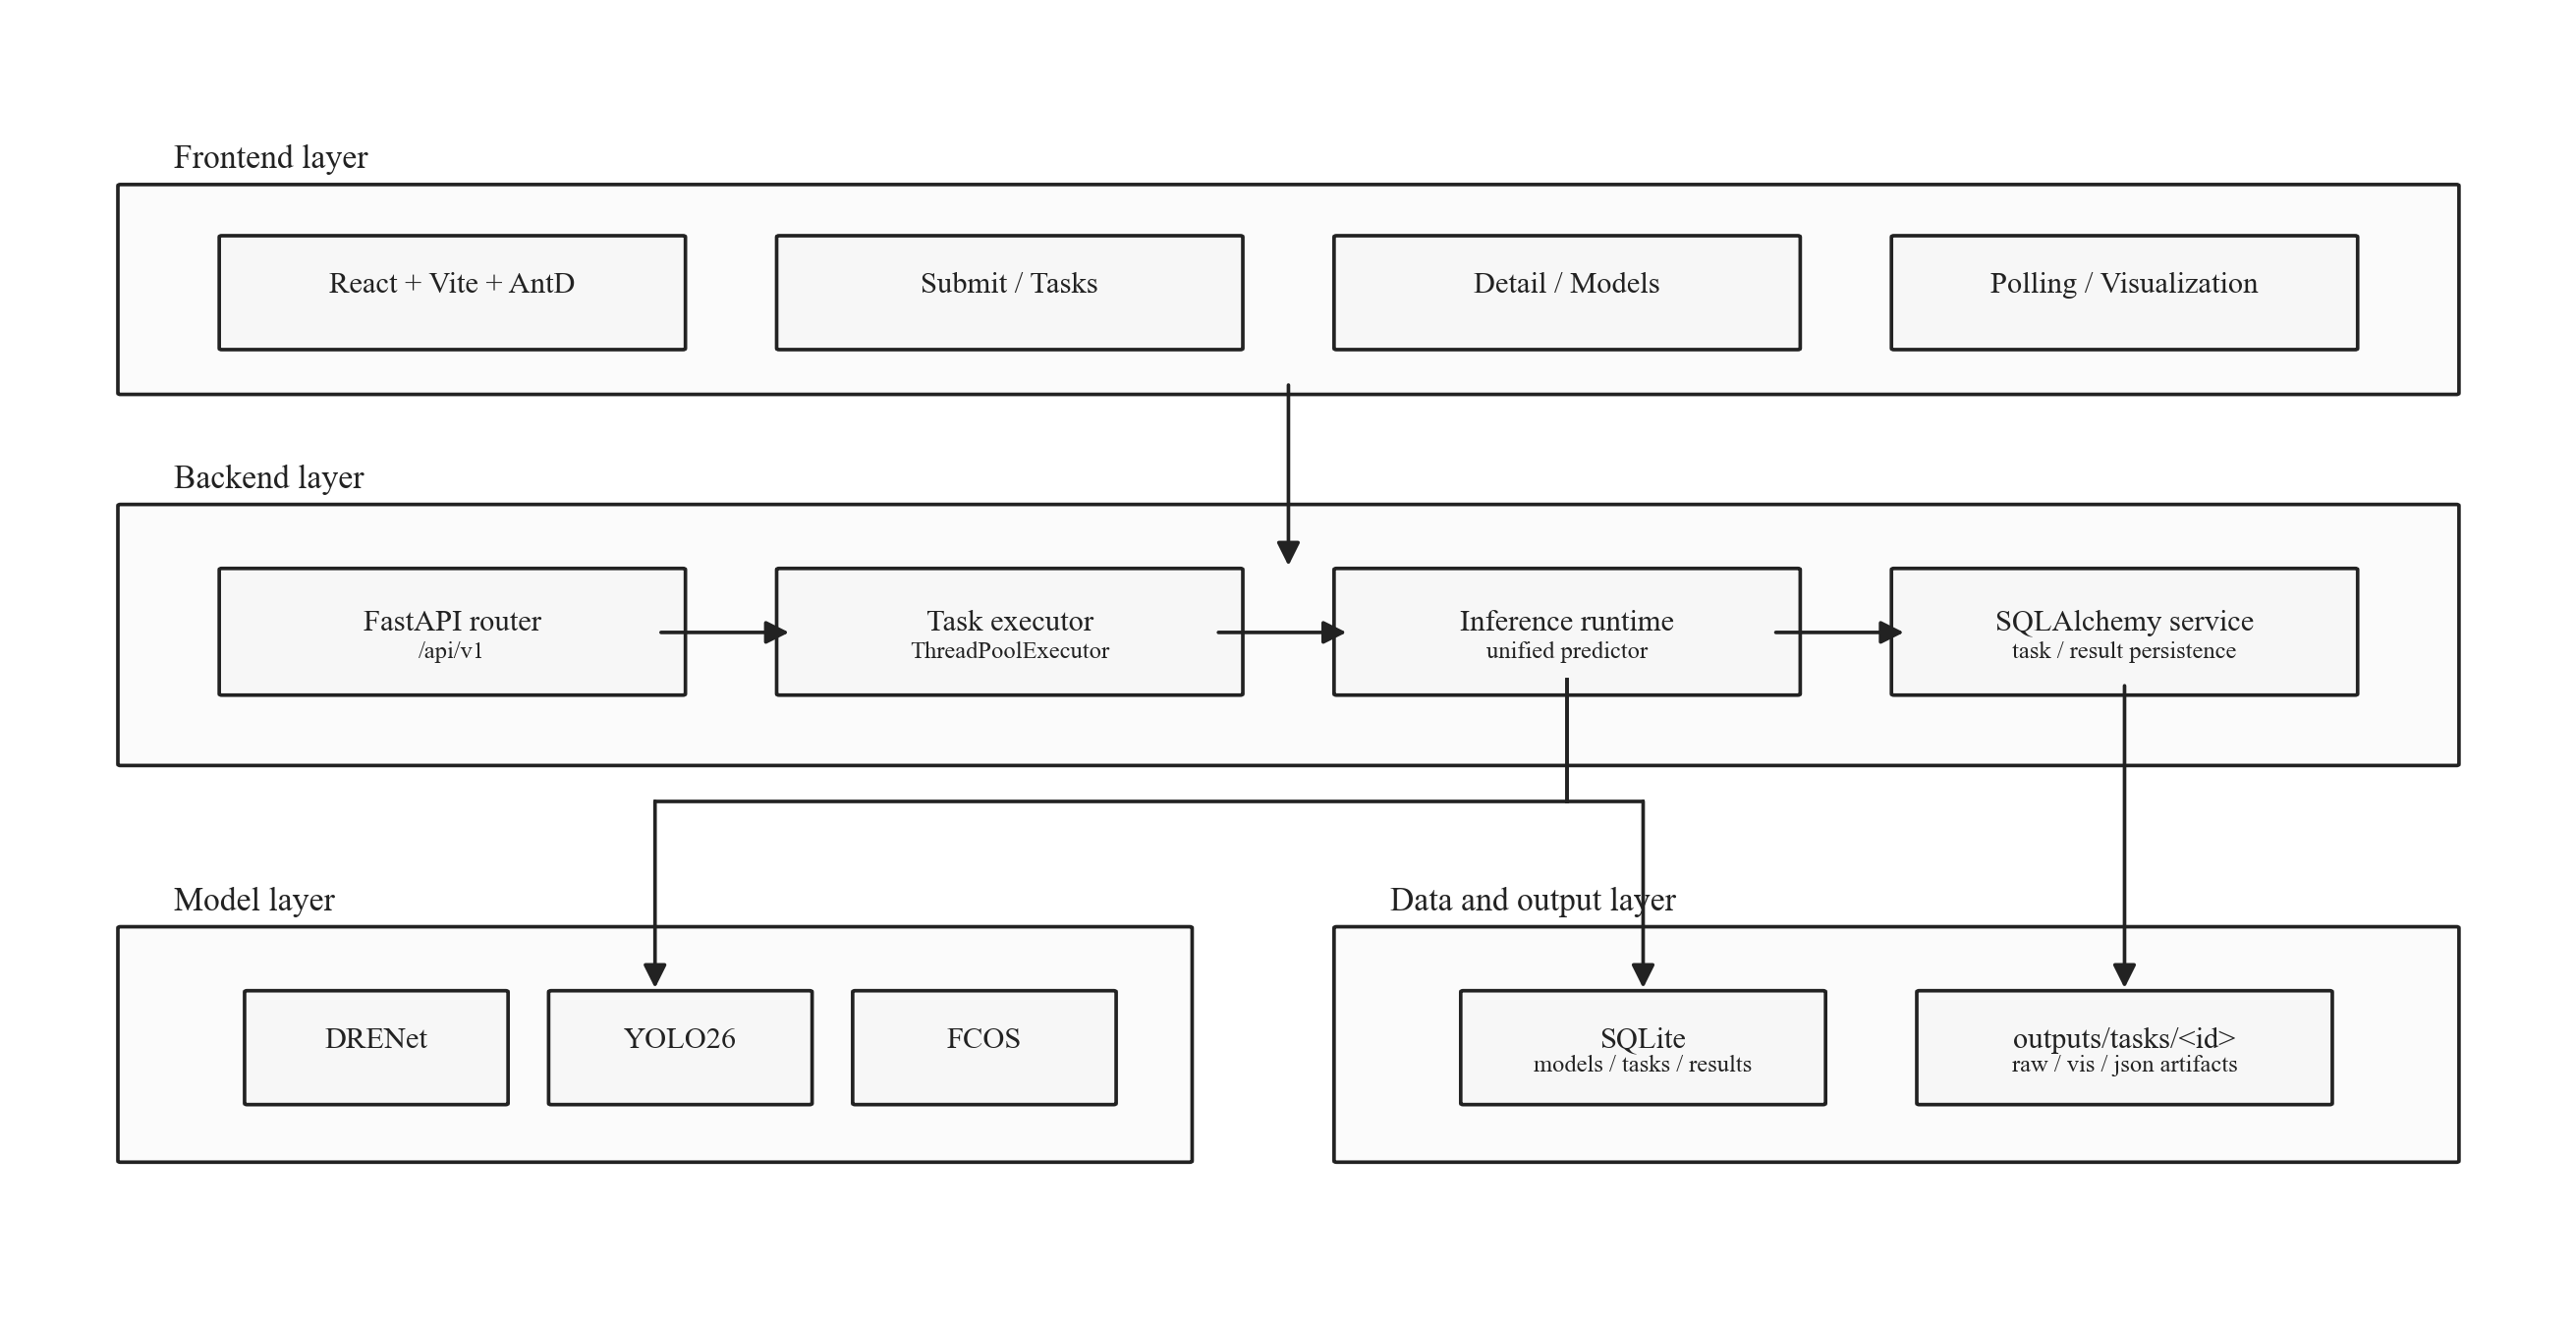
\includegraphics[width=0.96\textwidth]{img/ch5_architecture.png}
  \caption{系统总体架构示意}
  \label{fig:ch5_architecture}
\end{figure}

从职责划分角度看，系统可分为以下五层：

\begin{enumerate}
  \item \textbf{前端展示层}：基于 React、Vite、TypeScript 与 Ant Design，实现任务提交页、任务列表页、任务详情页和模型管理页；
  \item \textbf{后端服务层}：基于 FastAPI 提供任务提交、任务查询、结果查询、模型查询和健康检查等接口；
  \item \textbf{任务调度层}：基于 \texttt{ThreadPoolExecutor} 实现本地异步任务执行，降低界面阻塞与显存冲突风险；
  \item \textbf{数据持久化层}：基于 SQLite 与 SQLAlchemy 保存模型信息、任务状态、检测结果与文件路径；
  \item \textbf{算法能力层}：复用现有 \texttt{src/} 目录中的预测服务、模型适配器与融合逻辑，实现单模型与融合模式推理。
\end{enumerate}

图~\ref{fig:ch5_architecture} 中的分层主要服务于联调。前端只和 HTTP 接口交互，不直接接触模型文件；后端通过统一推理入口调用 DRENet、YOLO 或融合逻辑；数据库和输出目录共同保存状态与产物路径。这样的结构在答辩演示时更稳定，后续替换模型时也可以优先修改算法能力层和配置。

\subsection{数据库设计}

数据库围绕任务追踪和结果回看设计，核心表包括 \texttt{models}、\texttt{tasks}、\texttt{results} 和 \texttt{task\_files}。\texttt{models} 表保存模型名称、键值、权重路径和启停状态；\texttt{tasks} 表记录任务类型、执行模式、状态和时间；\texttt{results} 表保存检测框结构化结果；\texttt{task\_files} 表记录输入图、输出 JSON 和可视化结果路径。

\begin{figure}[htbp]
  \centering
  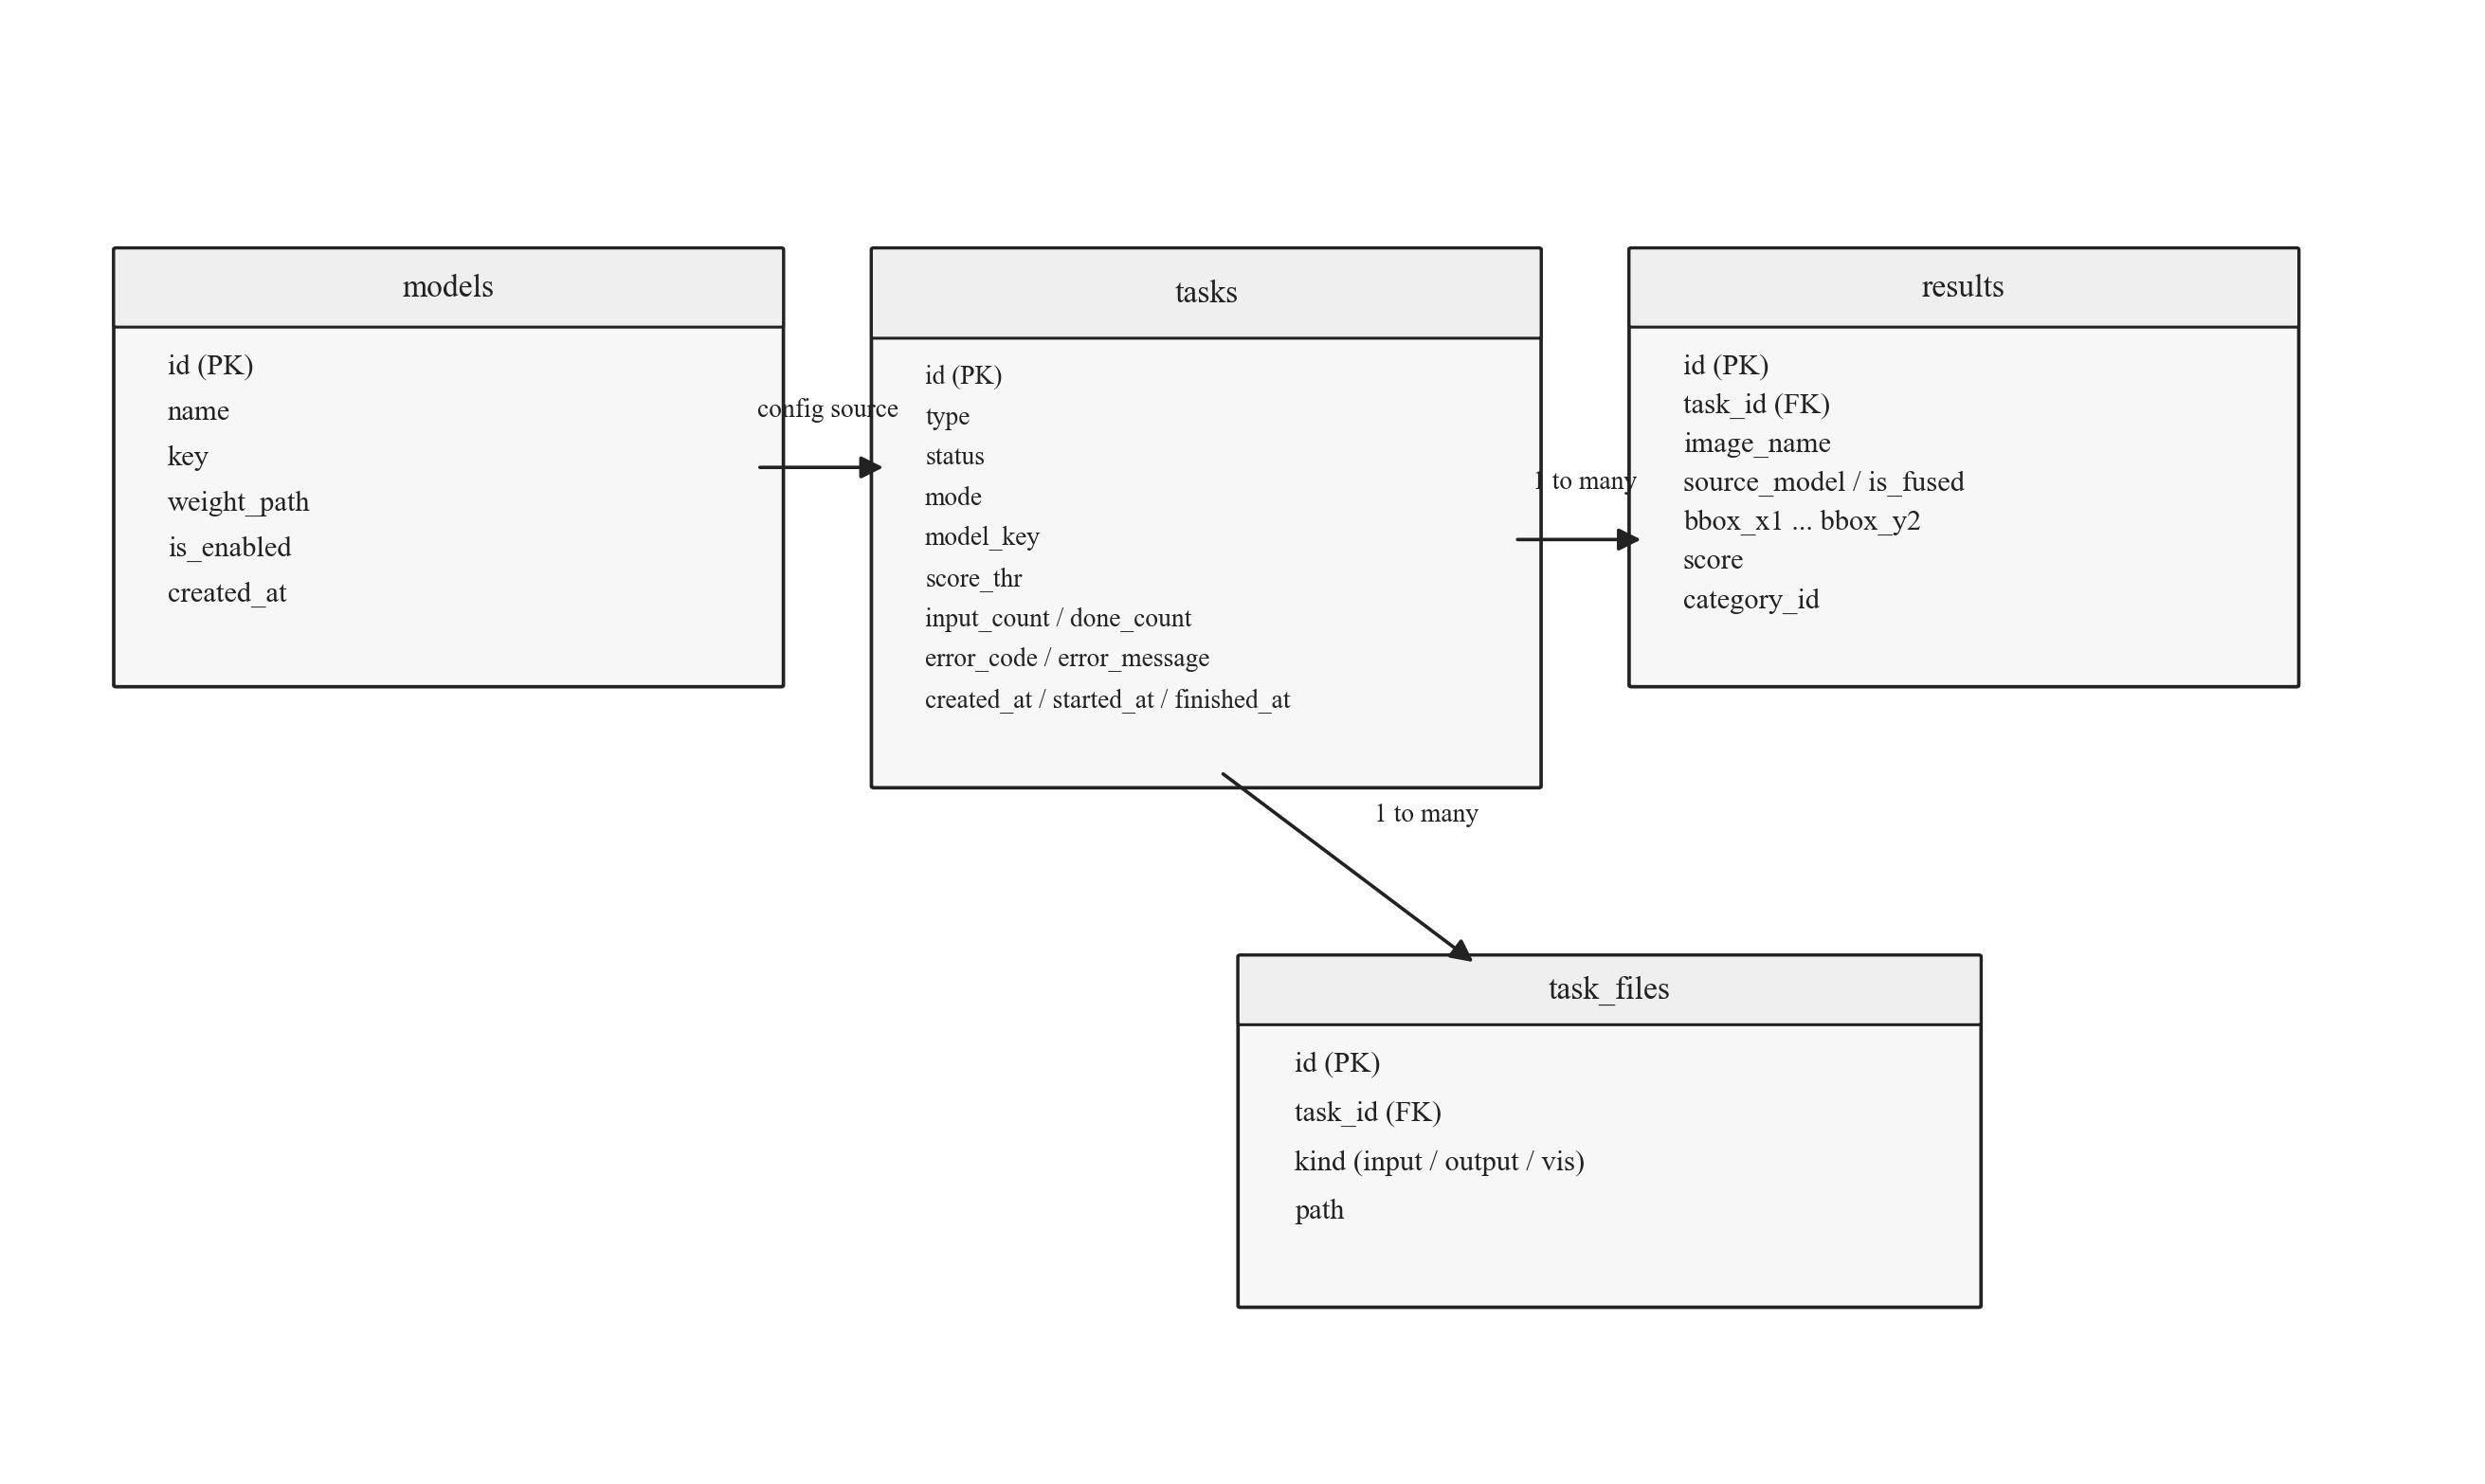
\includegraphics[width=0.94\textwidth]{img/ch5_er.png}
  \caption{系统数据库设计示意}
  \label{fig:ch5_er}
\end{figure}

图~\ref{fig:ch5_er} 展示了四张表之间的关系。\texttt{tasks} 表位于任务链路中心，一条任务可以对应多条检测框结果，也可以对应多个输入或输出文件记录。\texttt{models} 表同时服务前端模型管理页和后端推理校验。数据库没有引入用户权限、多租户等实体，因为这些功能对本文演示目标帮助不大，反而会增加实现复杂度。

\subsection{接口设计}

后端接口挂载在 \texttt{/api/v1} 路径下，主要接口见表~\ref{tab:ch5_api}。

\begin{table}[htbp]
  \centering
  \caption{系统核心接口设计}
  \label{tab:ch5_api}
  \small
  \begin{tabular}{>{\raggedright\arraybackslash}p{3.3cm}>{\raggedright\arraybackslash}p{1.8cm}>{\raggedright\arraybackslash}p{7.7cm}}
    \toprule
    接口路径 & 请求方式 & 功能说明 \\
    \midrule
    \path{/api/v1/tasks/infer} & POST & 提交单图或批量推理任务，返回任务编号与初始状态 \\
    \path{/api/v1/tasks} & GET & 查询任务列表、状态、进度与时间信息 \\
    \path{/api/v1/tasks/<task_id>} & GET & 查询单个任务的参数、状态与错误信息 \\
    \path{/api/v1/tasks/<task_id>/progress} & GET & 查询轻量级任务进度，仅返回状态与完成计数，用于高频轮询 \\
    \path{/api/v1/tasks/<task_id>/results} & GET & 查询任务结果、可视化文件路径和结构化检测框 \\
    \path{/api/v1/models} & GET & 查询模型列表与启停状态 \\
    \path{/api/v1/models/<model_key>} & PATCH & 更新模型启停状态 \\
    \path{/api/v1/health} & GET & 查询服务健康状态与模型加载情况 \\
    \bottomrule
  \end{tabular}
\end{table}

接口设计只保留真实运行和答辩演示必需的部分，包括任务提交、任务查询、结果查询、模型查询和健康检查。鉴权、复杂权限控制和跨节点调度暂不引入。这样做可以把精力集中在模型推理、任务状态和结果回看这些与课题最相关的功能上。

\subsection{关键实现流程}

\subsubsection{任务创建与执行流程}

任务从前端上传图像开始。用户选择模式、模型和阈值后，前端调用 \path{/api/v1/tasks/infer}。后端先校验图像、阈值和模型配置，再创建任务记录并写入数据库。之后任务进入本地线程池执行器，由执行器根据参数选择单模型或融合模式，并调用统一推理接口完成检测。

任务状态被明确记录为 \texttt{queued}、\texttt{running}、\texttt{done} 和 \texttt{failed}。前端列表页和详情页都读取这些状态展示任务生命周期；推理或文件处理出错时，后端会把错误信息写回任务记录，便于定位失败原因。

\subsubsection{结果生成与展示流程}

推理完成后，结构化检测结果写入数据库，输入图、输出 JSON 和可视化图像保存到 \texttt{outputs/tasks/<task\_id>/}。任务运行期间，前端优先轮询轻量级 \path{/api/v1/tasks/<task_id>/progress} 接口，只获取 \texttt{status}、\texttt{done\_count} 和 \texttt{input\_count} 等字段；任务结束后，再请求结果接口加载完整检测框和可视化产物。这样可以减少运行期间的大响应请求，同时保持进度条更新。

\begin{figure}[htbp]
  \centering
  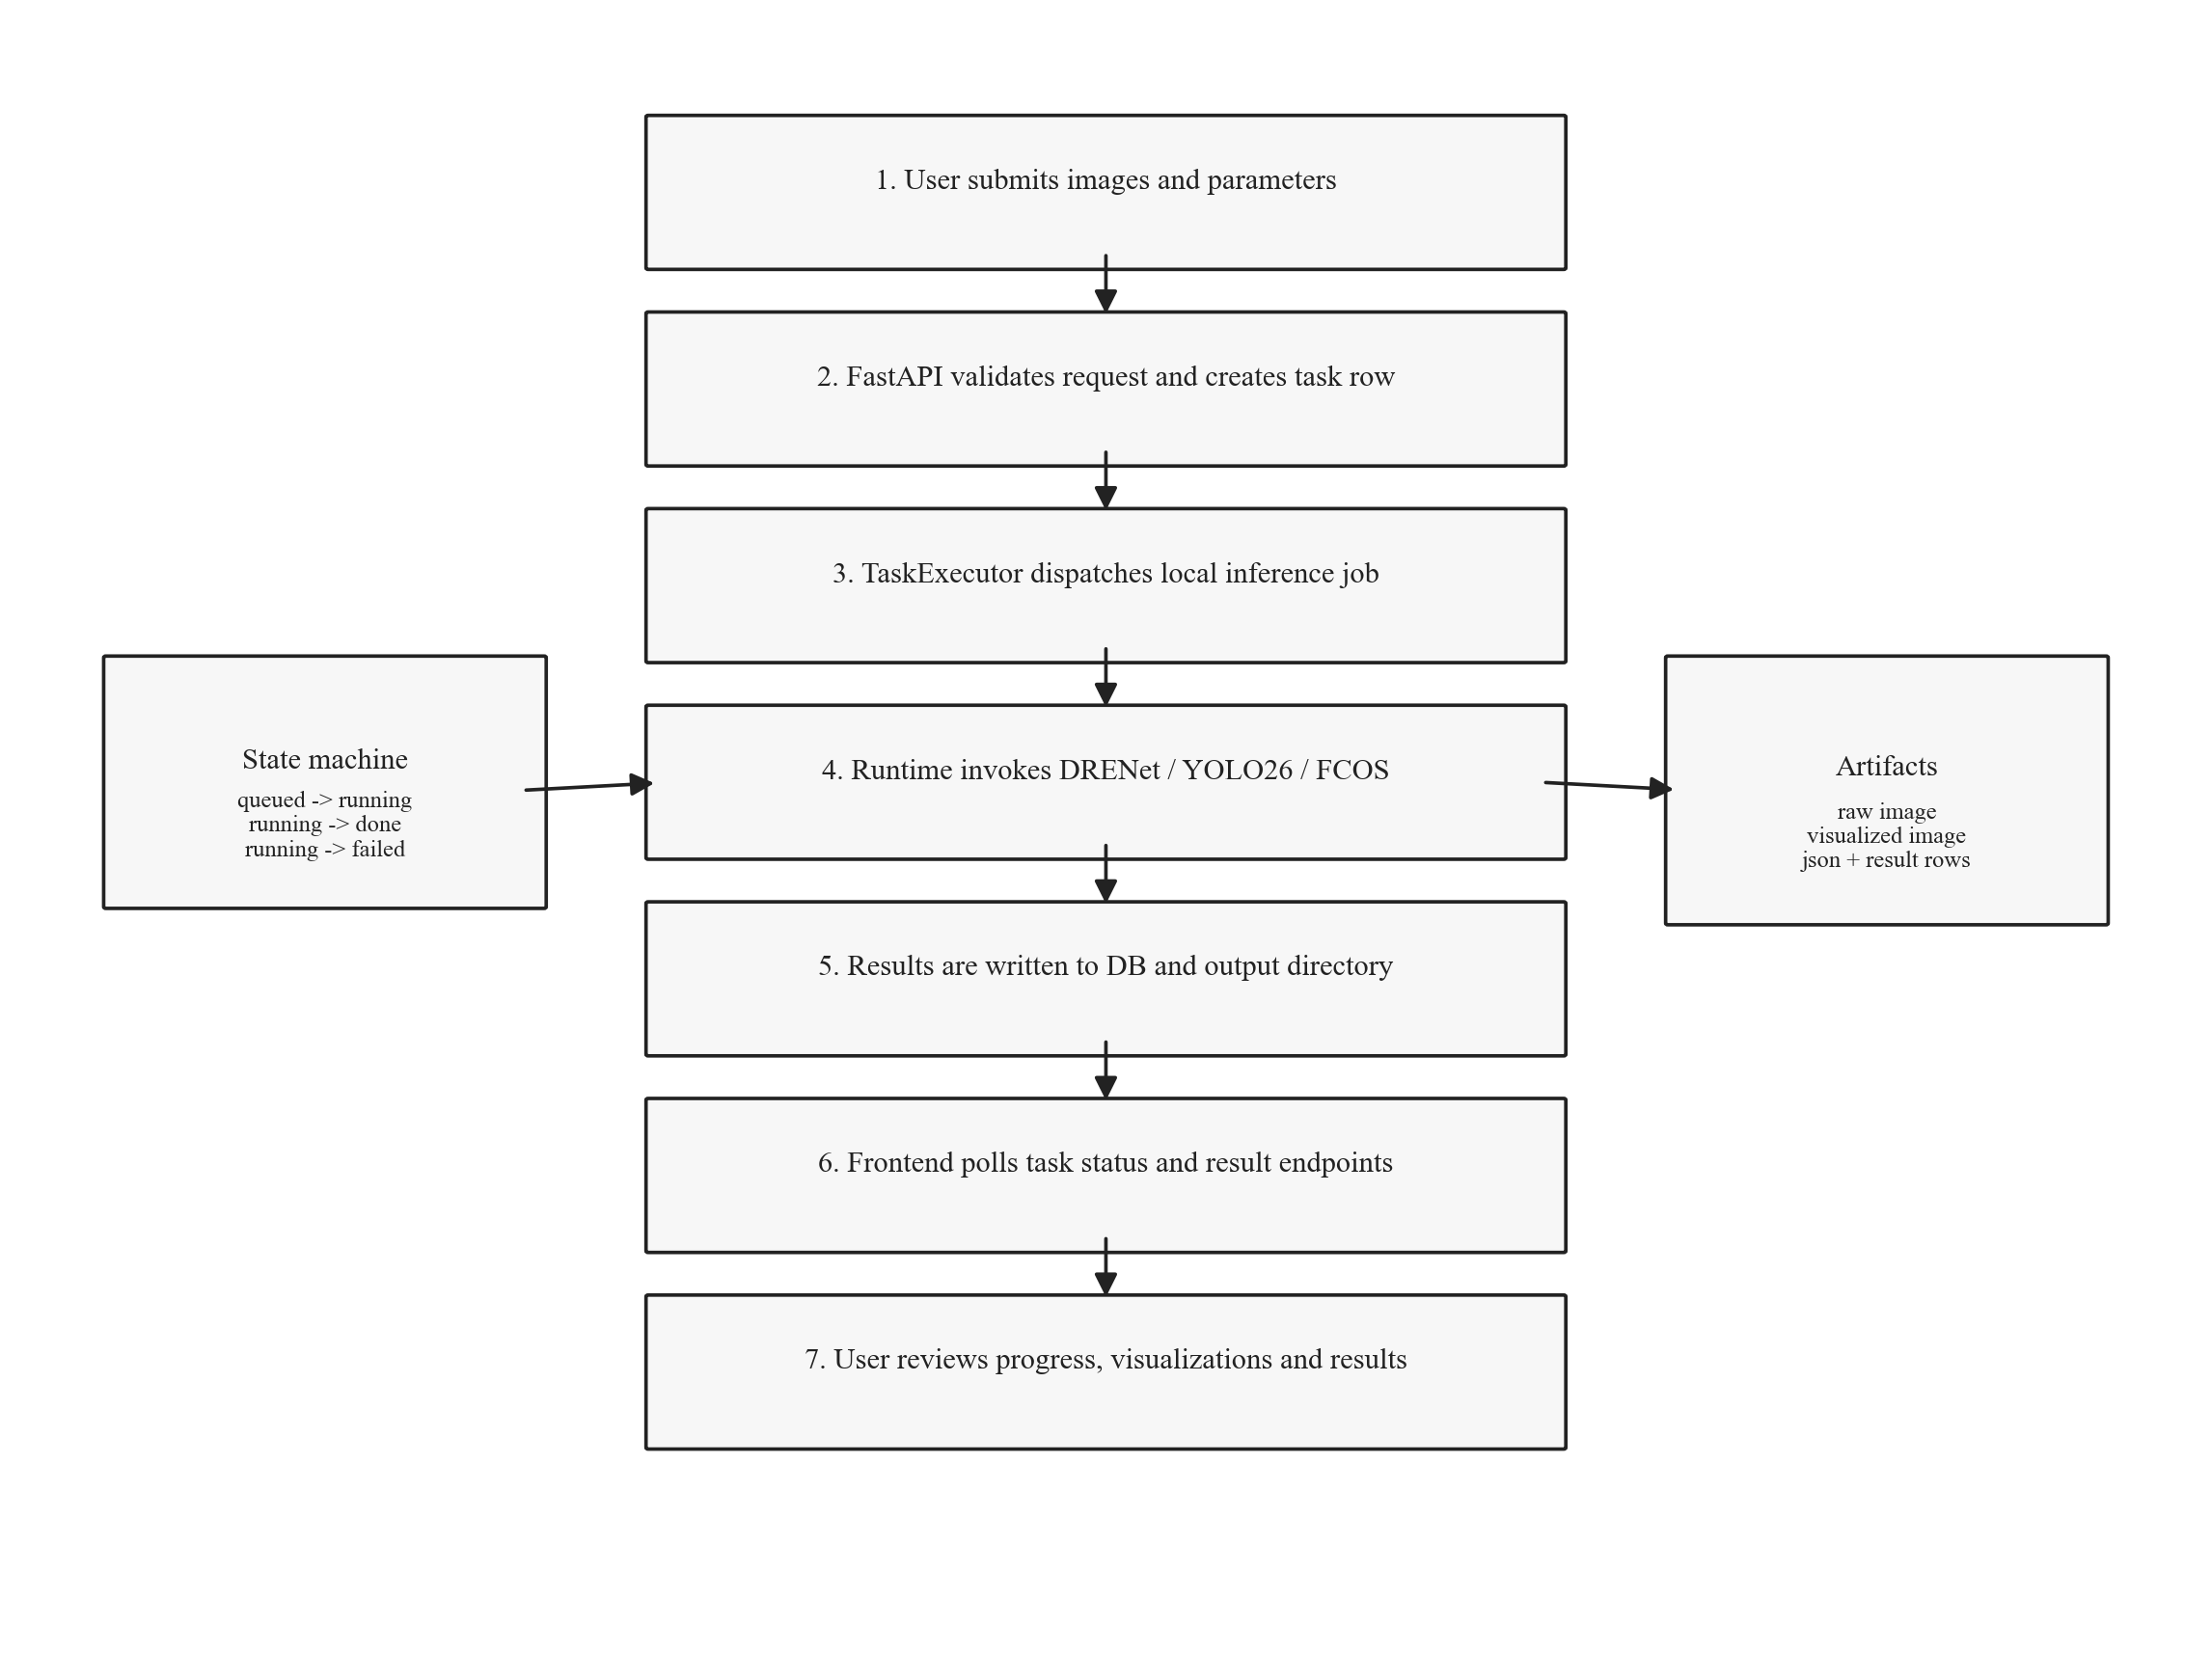
\includegraphics[width=0.88\textwidth]{img/ch5_flow.png}
  \caption{系统关键流程示意}
  \label{fig:ch5_flow}
\end{figure}

\subsection{系统实现效果与工程取舍}

经过前后端联调和真实模型接入测试，系统已经跑通任务创建、推理执行、结果保存和历史回放。当前系统可以接入 DRENet 与 YOLO 权重，完成单图和批量推理；任务列表支持轮询刷新、进度展示和失败状态标记；详情页展示模型来源、检测框、平均置信度和统计图表；结构化检测结果可以导出 CSV。SQLite 保存历史任务和检测结果，系统重启后仍可查询。

\subsubsection{前端页面实现效果}

页面设计围绕答辩演示组织。任务提交页支持单图和批量输入，推理模式、模型选择和阈值参数放在同一表单区域，减少演示时来回跳转。任务列表页突出状态、进度、模式、创建时间和耗时，方便快速判断系统是否正在运行。任务详情页展示可视化结果、检测框表格、模型来源和统计图表，用于回看单次任务的输入、执行和输出。

相比只展示一张检测结果图，Web 前端可以同时放置任务参数、执行状态、结果图像和结构化检测框。这样，论文中的实验结论不只停留在表格和文字中，也能通过系统任务记录进行复查。对毕业设计答辩来说，这比单纯展示截图更有说服力。

\begin{figure}[htbp]
  \centering
  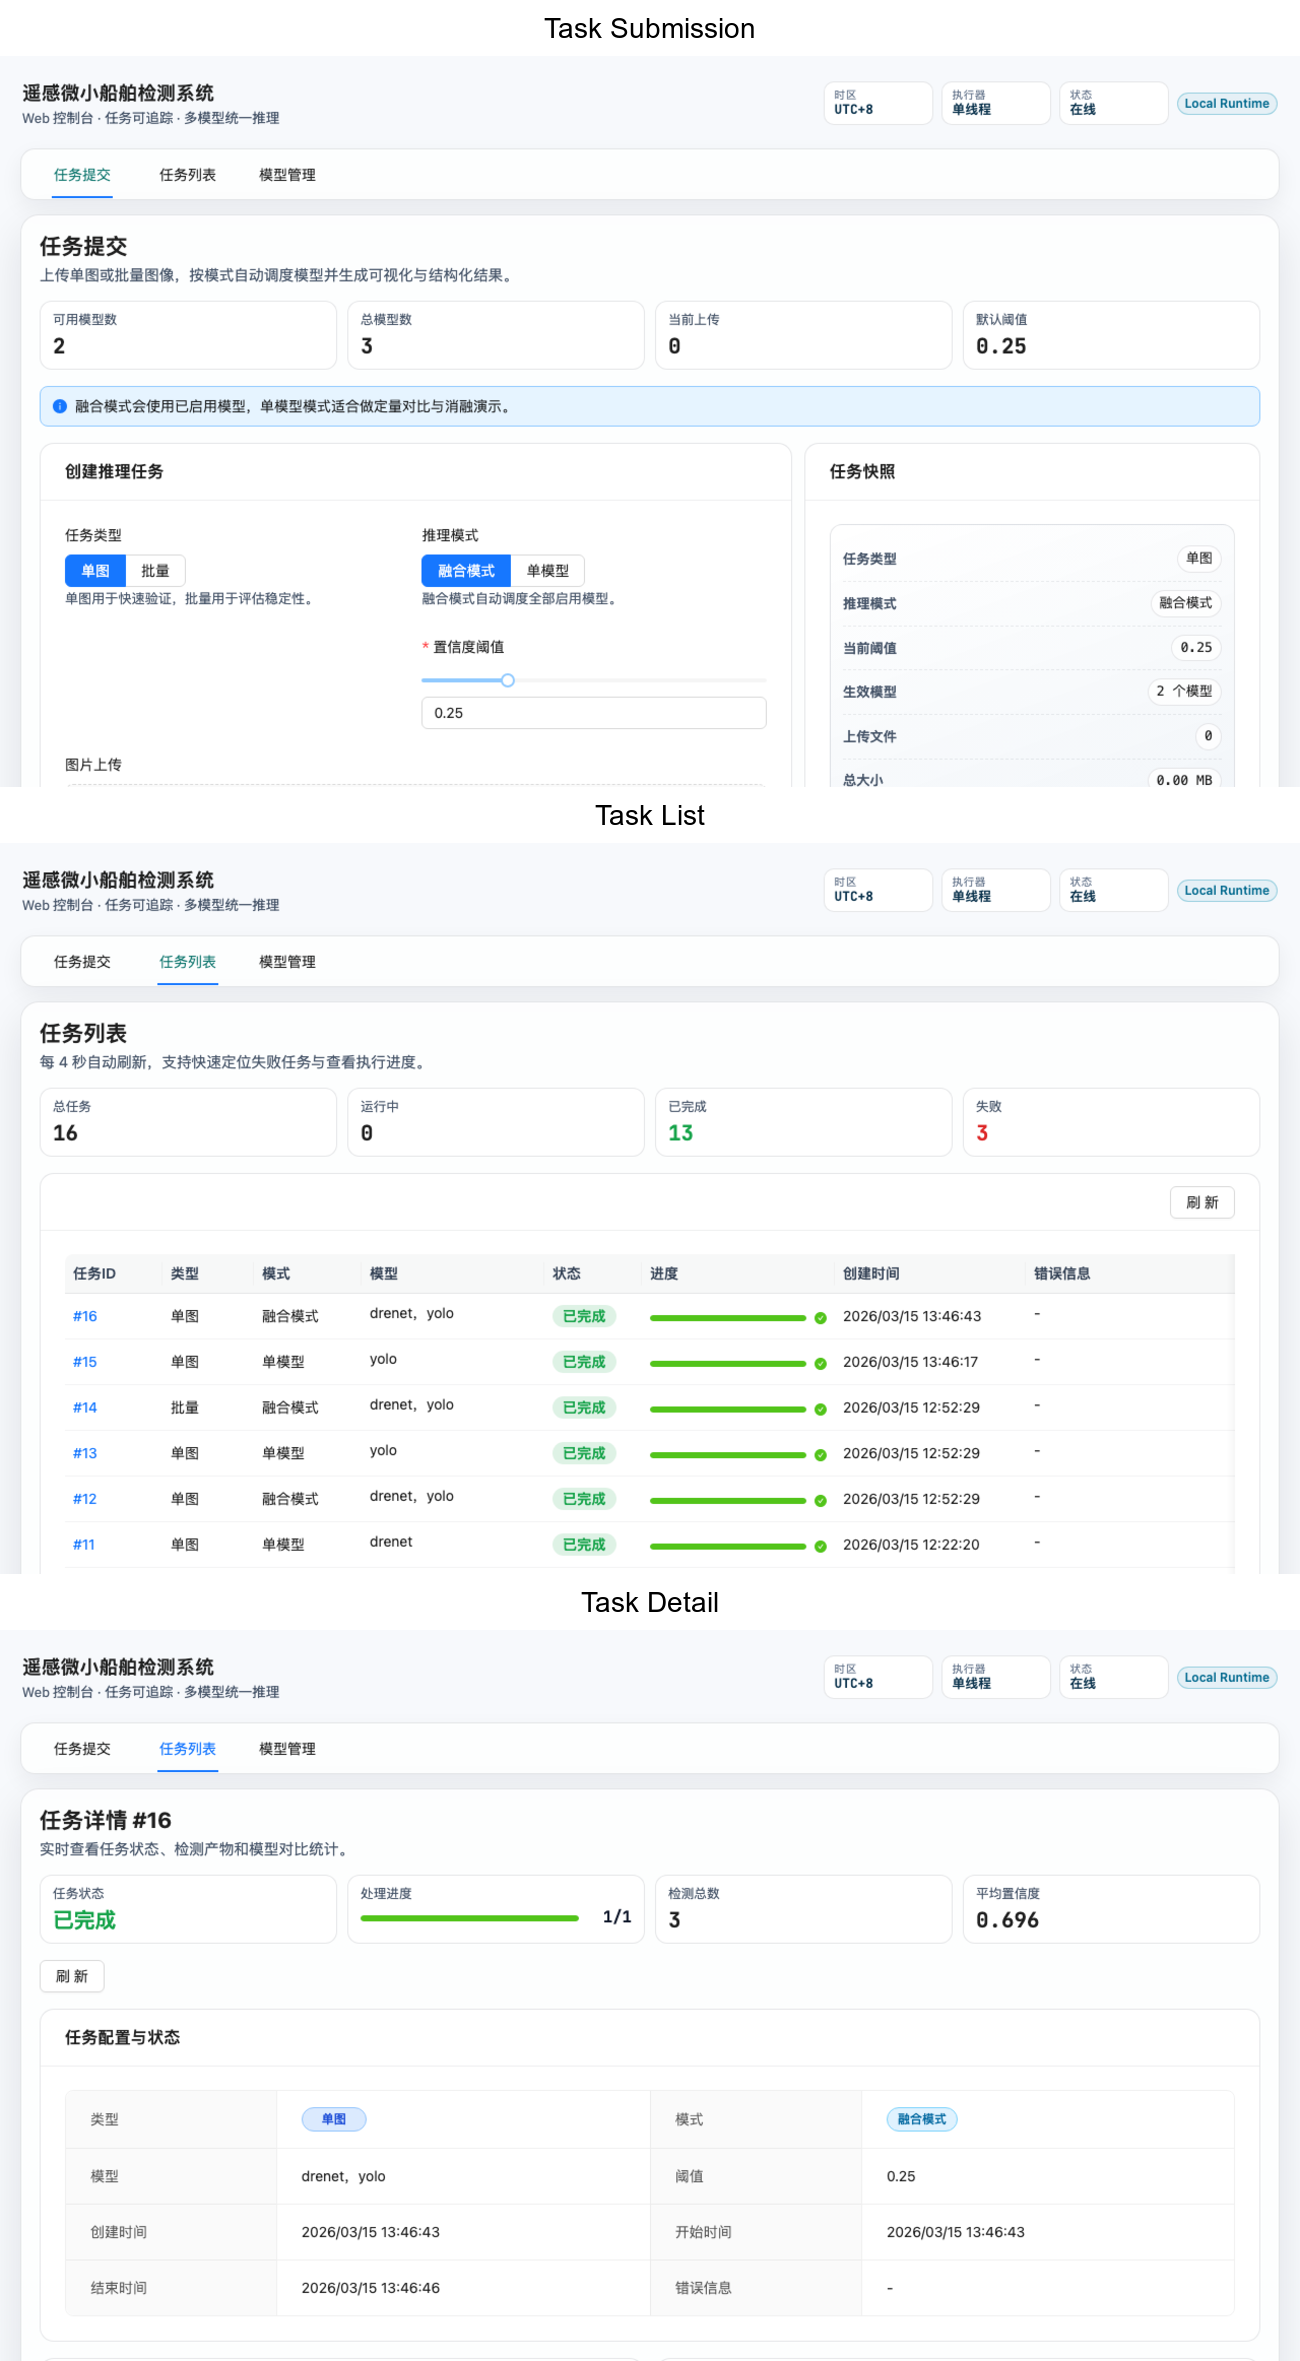
\includegraphics[width=0.76\textwidth]{img/ch5_pages.png}
  \caption{系统主要页面实现效果}
  \label{fig:ch5_pages}
\end{figure}

\subsection{系统响应速度优化}

系统联调时出现过一个比较明显的现象：模型本身推理并不慢，但前端页面上看到结果的时间要长不少。排查后发现，等待时间并不主要花在检测模型上，而是分散在融合模式串行调用、重复图像解码、运行期间拉取完整结果、数据库频繁提交和结果接口重复解析等环节。因此，本文把优化重点放在端到端响应时间上，而不是只看单个模型函数的耗时。

\subsubsection{性能瓶颈分析与优化思路}

沿着任务提交、推理执行和结果展示三段流程检查后，主要开销集中在七处：融合模式下多模型默认串行；任务运行期间前端反复请求完整结果；可视化阶段对同一张大图多次执行 \texttt{Image.open}；批量任务逐图提交数据库事务；结果接口重复解析数据集信息和参考框；任务输入阶段复制源图；首次推理时才加载模型权重。

对应改动也按这几处展开：融合推理增加可配置并行；前端轮询改为轻量 progress 接口；可视化阶段复用 \texttt{PIL.Image} 对象；批量任务改为分段提交；数据集信息和参考框加入内存缓存；输入文件优先使用符号链接；应用启动时预加载启用模型。这些改动的共同目标是减少“推理之外”的等待，而不是把系统改成更复杂的工程架构。

\subsubsection{并行推理与模型预加载机制}

融合模式需要对同一张图像调用多个模型，再合并检测结果。原始实现按顺序执行，总耗时接近各模型耗时之和。为减少这部分等待，后端推理运行时加入基于 \texttt{ThreadPoolExecutor} 的并行推理机制，并通过环境配置控制并行模型数。并行度设为 1 时仍按串行执行；GPU 资源较充足时，可以提高并行度来缩短融合推理时间。

并行并没有被设为默认开启。原因是本地 CPU 环境下线程争抢会使单模型耗时上升；GPU 环境下三模型并行虽然可能提速，也可能带来显存竞争。本文因此保留默认并行度为 1，只在资源允许时手动提高并行度，让系统在不同机器上更容易稳定运行。

此外，系统在 \texttt{startup} 阶段预加载已启用模型权重，避免第一次提交任务时才初始化模型。这个改动不改变稳态吞吐量，但能去掉首次推理的额外等待，对答辩演示比较有用。

\subsubsection{轻量级进度端点与前端轮询重构}

优化前，任务详情页每 4 秒轮询一次，并同时请求任务详情和完整结果。实现上很简单，但体验不理想：任务实际完成后，页面最多还要等 4 秒才刷新；任务运行期间反复请求结果接口，也会产生不必要的数据传输和后端解析开销。

为此，后端新增轻量级进度接口，只返回 \texttt{status}、\texttt{done\_count} 和 \texttt{input\_count} 等字段。前端改为两阶段轮询：任务处于 \texttt{running} 时，每 1.5 秒请求 progress 接口，只更新进度条和状态；任务转为 \texttt{done} 或 \texttt{failed} 后，再请求结果接口加载完整检测数据和可视化产物。高频轮询响应由约 25KB 缩减到约 64B，页面感知延迟也随之降低。

\subsubsection{渲染、存储与结果访问优化}

可视化渲染阶段原先会多次打开同一张图。本文扩展了 \texttt{render\_detections()} 的输入方式，使其既能接收图像路径，也能直接接收 \texttt{PIL.Image} 对象。融合模式下，系统只需打开一次原始图像，就能复用到多个模型结果和融合结果的渲染中。

批量任务中，数据库提交策略也做了调整。原先每处理一张图就立即提交，现在改为每处理两张图或到达任务末尾时提交一次。这样既保留阶段性进度，又减少事务提交次数。结果接口另外加入数据集信息和参考框缓存，避免同一张图片多次查询时重复遍历目录和解析标注。

输入文件准备阶段优先使用符号链接代替物理复制，以减少大图 I/O；如果符号链接创建失败，再回退到复制方案。上述改动都不复杂，但能一起缩短任务从提交到结果展示之间的实际等待。

\subsubsection{优化效果分析}

为检查这些改动是否有效，本文在本机环境下对几个关键环节做了微基准测试，结果见表~\ref{tab:ch5_perf}。

\begin{table}[htbp]
  \centering
  \small
  \caption{系统响应速度优化的关键基准结果}
  \label{tab:ch5_perf}
  \begin{tabular}{p{3.0cm}p{2.2cm}p{2.2cm}p{2.0cm}p{4.0cm}}
    \toprule
    优化项 & 优化前 & 优化后 & 提升倍数 & 说明 \\
    \midrule
    三模型融合推理 & 465.6 ms & 156.2 ms & 2.98$\times$ & mock 模式下，3 workers 并行相对串行 \\
    前端结果可感知延迟 & 4.0 s & 1.5 s & 2.67$\times$ & 运行期间改为轻量 progress 轮询 \\
    大图可视化渲染 & 443.9 ms & 336.1 ms & 1.32$\times$ & 4096$\times$4096 图像由 4 次解码降为 1 次 \\
    批量任务数据库提交 & 62.6 ms & 37.6 ms & 1.66$\times$ & 10 张图任务由逐图提交改为分段提交 \\
    输入文件准备 & 2.4 ms & 0.8 ms & 3.00$\times$ & 优先 symlink，失败时回退 copy \\
    \bottomrule
  \end{tabular}
\end{table}

表~\ref{tab:ch5_perf} 中的收益主要来自两类变化：一是减少串行等待，例如融合推理并行和轻量 progress 轮询；二是减少重复工作，例如图像复用、结果缓存和分段提交。需要注意，部分数据来自 mock 或微基准场景，不能直接等同于生产环境吞吐量。但这些结果和实际联调中的页面响应改善方向一致，足以说明优化思路是有效的。

工程取舍上，本文没有引入消息队列、分布式任务系统或独立数据库服务器，而是保持本地单机架构。这个选择并不是忽略工程能力，而是考虑到毕业设计的时间、部署环境和答辩演示需求。单机方案已经能覆盖前端、后端、数据库和算法集成，复杂度也更容易控制。

任务调度也沿用这一取舍。系统没有使用 Redis、Celery 等中间件，而是采用 \texttt{ThreadPoolExecutor} 实现本地异步执行，并叠加任务级异步和模型级可配置并行。对生产系统来说，它的扩展性不如分布式队列；但在当前场景下，它能降低显存冲突风险、部署复杂度和跨服务联调成本，同时保留任务状态、失败回写和性能调优所需的基本能力。

SQLite 的选用也是同样原因。本文引入数据库是为了保存任务记录、结果和产物索引，而不是模拟企业级数据库方案。对单机演示和历史回看来说，SQLite 的部署成本更低，维护也更简单。

\subsection{小结}

本章说明了系统建设目标、需求、架构、数据库、接口、任务流程和响应速度优化。系统已经在本地环境中跑通多模型接入、异步任务执行、结果持久化和前端展示，也能承接第四章中的部分实验结果。

从交付角度看，第五章不只是展示前后端页面，而是说明模型训练、离线评测、结果存储和在线展示已经被接到同一条链路上。实验表格、定性样例和系统任务详情可以互相核对，这也是系统部分相对于静态结果截图的价值。
